\subsection{Исследование профиля высвечивания сместителя спектра}\label{section:secWLS}

Анализ распределения во времени хитов, принадлежащих одному черенковскому кольцу, позволяет исследовать временные свойства сместителя спектра. Анализу подлежит распределение разностей временных отметок хитов каждого кольца относительно первого по времени хита в данном кольце. В зависимости от длины волны черенковский фотон может с той или иной вероятностью либо поглотиться сместителем спектра и вызвать его свечение, либо пройти сквозь слой сместителя спектра без взаимодействия и попасть фотокатод. В результате, даже при наличии слоя сместителя спектра, часть хитов подчиняются временной зависимости характерной для чистого ФЭУ.
%часть хитов подчиняЮтся или подчиняЕтся?
%Проверить пунктуацию
Таким образом, для получения кривой высвечивания сместителя спектра необходимо из распределения разностей времен, полученного со сместителем спектра, вычесть должным образом отнормированное в максимуме распределение разностей времен, полученное с чистым ФЭУ.

Нормированные в максимуме кривые высвечивания со сместителем спектра и без него показаны на рис.~\ref{fig:WLStwoCurves}, а разность этих распределений --- на рисунке~\ref{fig:WLSdiff}. Видно, что за исключением небольшой выпуклости в области 7~нс, связанной с особенностями работы (?данного семейства?) МА~ФЭУ, кривая выглядит похоже на сумму нескольких экспонент.
%Мне не нравится "похоже на"
%Вообще то эта выпуклость объясняется битыми каналами, наводками, а не чем-то, связанным с ФЭУ.

\begin{figure}
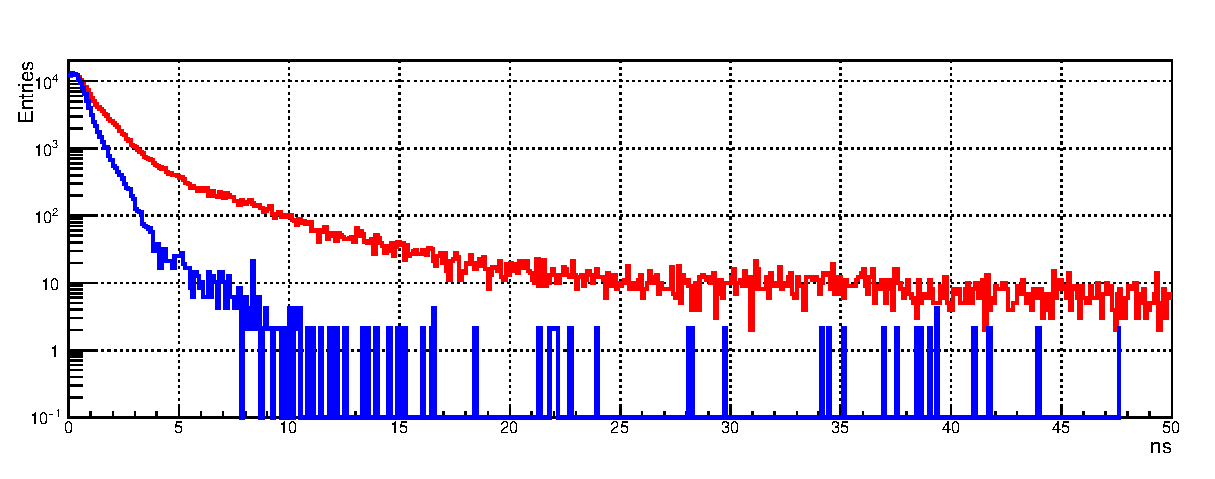
\includegraphics[width=1.0\textwidth]{pictures/WLS.eps}
\caption{Измеренные кривые высвечивания со сместителем спектра (красный, выше) и без него (синий, ниже).}
\label{fig:WLStwoCurves}
\end{figure}

\begin{figure}
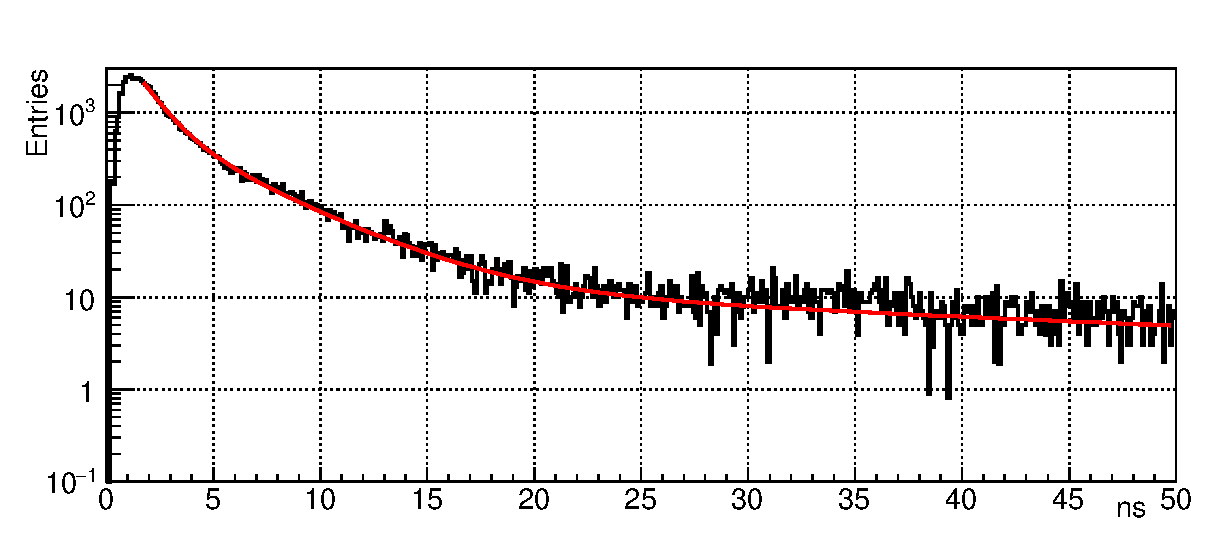
\includegraphics[width=1.0\textwidth]{pictures/WLSdiff_1Nov.eps}
\caption{}
\label{fig:WLSdiff}
\end{figure}

%Напрашивается вводное слово между двумя следующими предложениями.
Указанная выпуклость не позволяет надежно извлечь характерные времена высвечивания. Интересно сравнить полученную кривую с результатами флюориметрических исследований. Стеклянная пластина со слоем сместителя спектра, нанесенным точно таким же методом, как и на МА~ФЭУ, была исследована с помощью классического метода счета фотонов при возбуждении светом с длиной волны 280~нм. Были получены следующие значения времен высвечивания и относительные интенсивности~(\cite{DUERR}):

$ A_{1} \cdot e^{(-t / \tau_{1})} + A_{2} \cdot e^{(-t / \tau_{2})} + A_{3} \cdot e^{(-t / \tau_{3})}$

Подгонка кривой с риc.~\ref{fig:WLSdiff} суммой трех экспонент с соответствующими временами показывает разумное согласие. Получены следующие относительные вклады компонент: 


Отметим, что относительный вклад медленной компоненты оказывается ниже, чем в (?), что можно объяснить влиянием способа возбуждения на заселение разных типов центров высвечивания.

В пределе большого числа хитов в кольце использованный нами метод переходит в стандартный метод исследования флюоресценции путем счета единичных фотонов~\cite{}. Однако в нашем случае существует некоторая случайная задержка между моментом попадания черенковского фотона на поверхность МА~ФЭУ и временем прихода первого хита. С целью выявления влияния метода на измеренные времена высвечивания было проведено Монте Карло моделирование.

%Слово фит и его производные вообще употребимы в литературном языке?
В модели были заложены разброс времени прохода лавины в МА~ФЭУ 300~пс (RMS), три экспоненциальные компоненты с характерными временами ???, ???, и ??? и соответствующими амплитудами ???, ???, ???. Получившееся распределение и его фит тремя экспонентами со свободными параметрами показаны на рис.~\ref{}. Если начать область фитирования, отступив ???, разброс времени прохождения лавины величины постоянных распада экспонент воспроизводятся с точностью лучше ???\%, а соответствующие амплитуды несколько искажаются, что естественно, поскольку исследуется область отстоящая на ???~нс от начала импульса.

Практическая ценность проведенного исследования состоит в том, что может быть оптимизирована длительность окна, в пределах которого хиты принимаются одновременными и могут быть приписаны одному кольцу (?то есть событию, что более правильно, т.к. в событии будет несколько колец и вообще, с т.з. полного эксперимента рассматривается задача построения события?). Для этого необходимо найти баланс между числом дополнительных хитов, полученных благодаря сместителю спектра и вероятностью наложения сигналов друг на друга или подхвата в кольцо темнового хита.
%Што?
Например, прирост хитов в 15\% может быть достигнут при длительности окна 15~нс?